\section{The TSTL Harness Language}

The TSTL compiler takes as input a harness template file, and produces
as output a Python class file that implements an interface other tools
can use to perform testing on the SUT via an SUT-independent interface.

The harness in Figure \ref{fig:MakeFeatureLayer} shows many of the
basic features of TSTL.  The basic structure of a TSTL harness
consists of three parts, usually written in order.  First, harness
code prefixed by an {\tt @} or enclosed in {\tt <@ @>} is treated as
raw Python code, and essentially not interpreted by the TSTL
compiler.  This code is reproduced almost literally in the output
file\footnote{TSTL does have to scan {\tt import}s to re-load modules, and also pre-processes function
  definitions to support
pre- and post-conditions.}.  Second, there is a preamble that almost
always defines a set of \emph{value pools} for use in testing, but
also may include information on logging, correctness properties,
source code locations for code coverage analysis, and other basic
information that applies to the entire harness.  Finally, the bulk of
a TSTL harness (and the only non-optional element) is a set of
\emph{action definitions}.  Actions are the possible steps to be taken in
testing, and define the set of possible tests.

The original version of TSTL \cite{NFM15} required cumbersome use of Python
functions to implement many simple operations, including guards.  Current TSTL extends
the language to make it possible to define very complex test spaces
using only pools and actions, with helper functions only required for
the usual reasons of abstraction and readabiliy.

\subsection{The Essentials of Pools and Actions}

In TSTL, tests usually consist of assignments to value pools and uses of the
values in those pools.  In order to make the core ideas clear,
consider part of Figure \ref{fig:MakeFeatureLayer}, defining how to
generate values used in SQL where clauses.  The following, by itself,
is a valid TSTL harness (albeit one that cannot discover any
interesting faults):

{\scriptsize
\begin{code}
pools:
  <val> 2 CONST
\vspace{0.05in}
actions:
\vspace{0.05in}
<val> := <1..10>
<val> = <val> + 1
\end{code}
}

There is only one pool, named {\tt val}.  The pool has room to store
two values.  The state of the SUT is defined by the state of all
pools.  Initially, all pools are set to a special value ({\tt None}) indicating the
pool has not been initialized.  Pools can be thought of as 
normal Python variables, for the most part, so we can think of the
{\tt val} pools as variables {\tt val0} and {\tt val1}.

Actions that include the {\tt :=} form of assignment (a TSTL, not
Python, operation) initialize pool values.  When {\tt <val>} appears
in an action, that represents all possible pool locations with that
name:  for our simple example, either {\tt val0} or {\tt val1}.  An
integer range is represented by {\tt <i..j>}, and TSTL expands such
ranges to produce an action with each possible choice. The
first line in the actions section of this harness translates to 20
different possible actions:

\begin{figure}
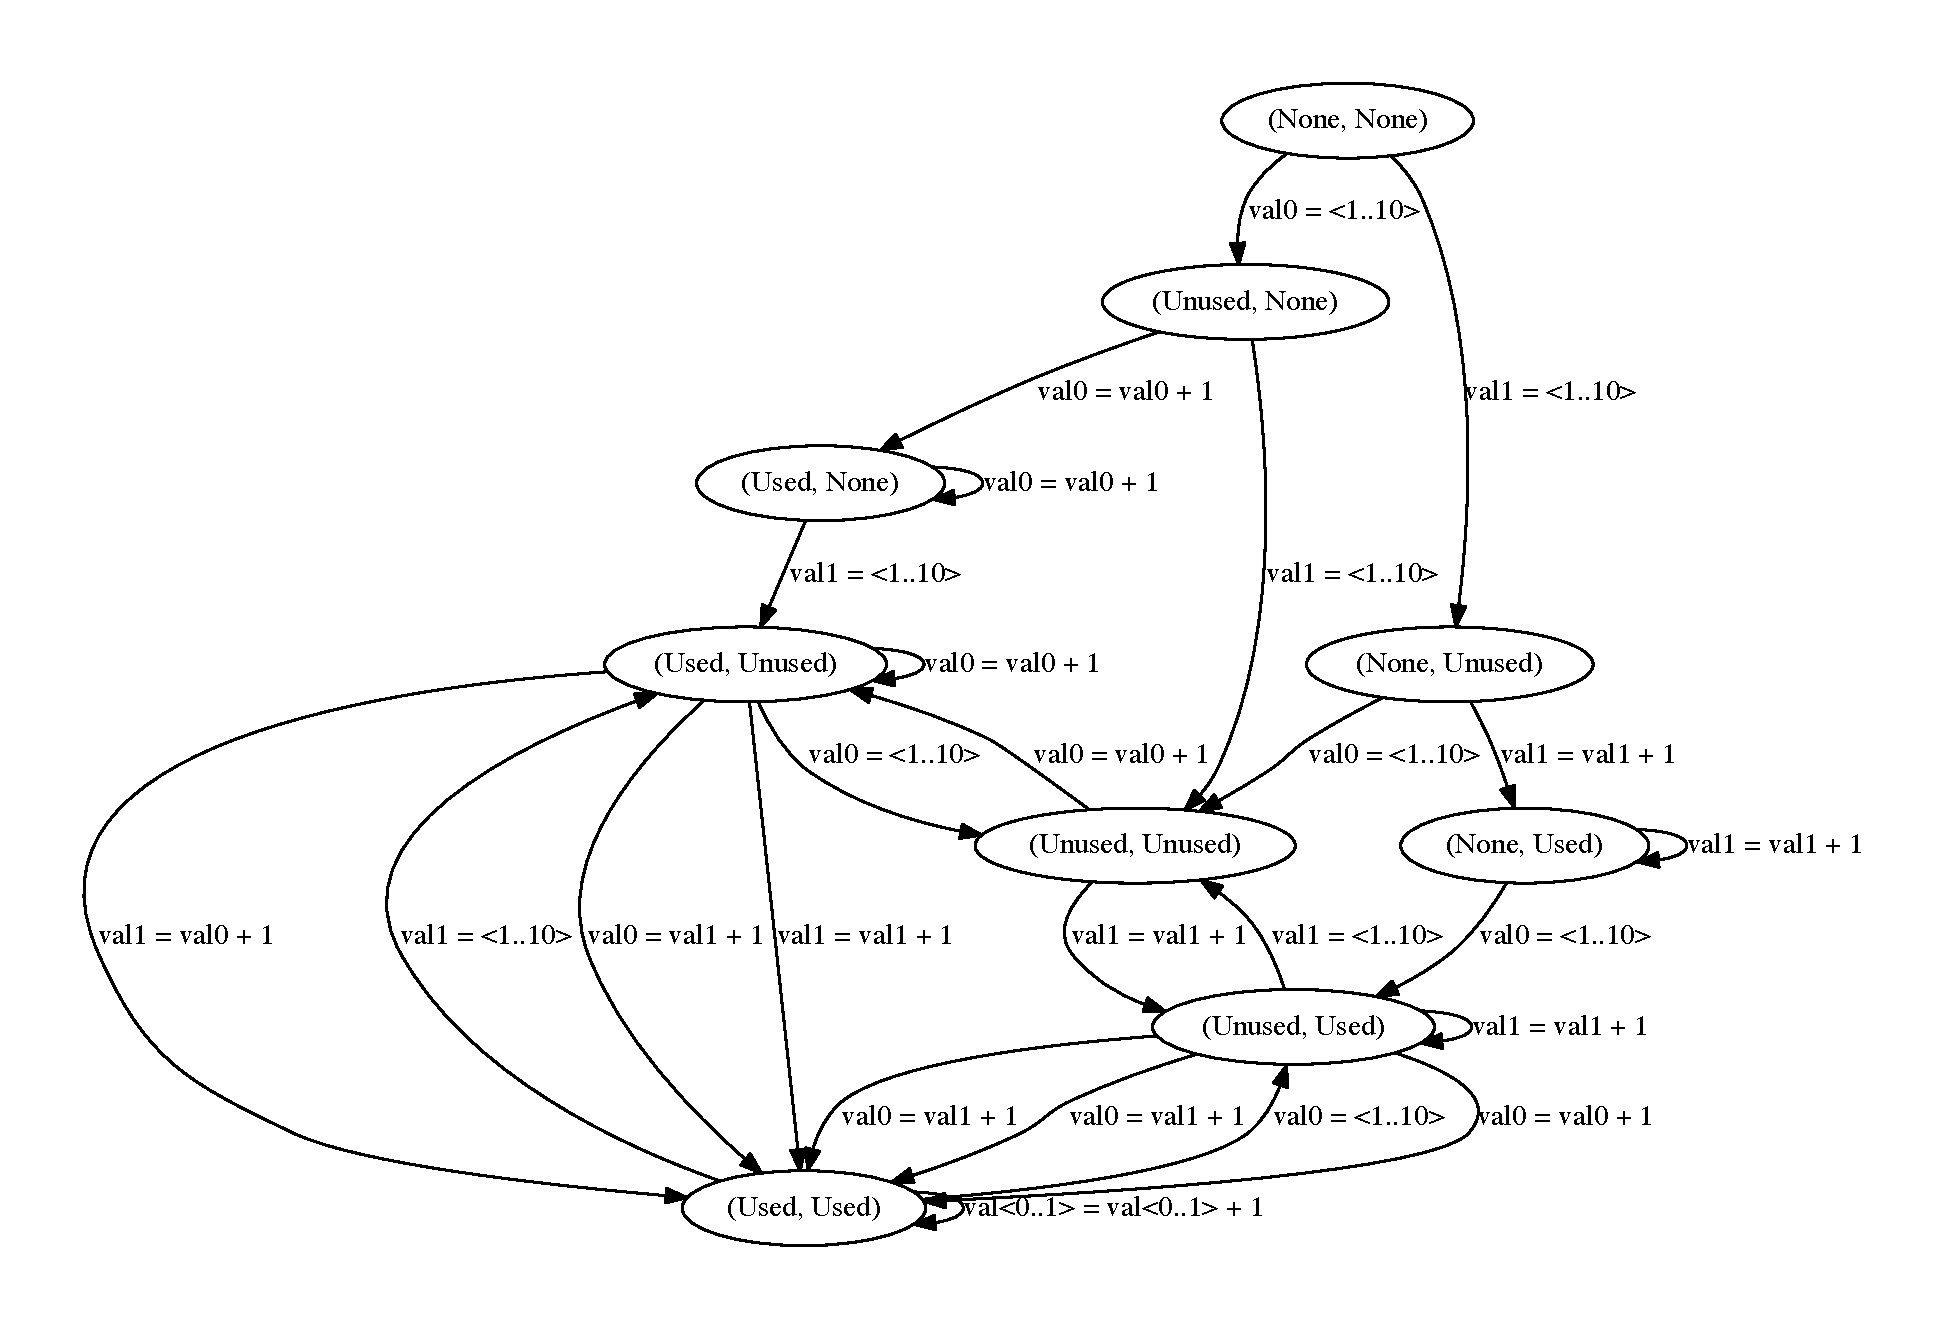
\includegraphics[width=\columnwidth]{states}
\caption{Constraints on actions in a test, based on pool states}
\label{fig:poolacts}
\end{figure}

{\scriptsize
\begin{code}
val0 = 1
val0 = 2 ...
val0 = 10
val1 = 1 ...
val1 = 10
\end{code}
}

From the initial state of the system, only these 20 actions are
\emph{enabled}.  The first concept that is essential to understanding
TSTL semantics is that at any state of the
system, the only actions that are enabled are those that do not
\emph{use} any non-initialized pool values.  Any appearance of a pool
value is a use, with the single exception of the left-hand-side of a
{\tt :=} initialization.  The second concept is that a value
cannot be initialized (appear on the lhs of {\tt :]}) until after at
least one action
that uses it has been executed.  Figure \ref{fig:poolacts} shows the
consequences of these rules for the simple value assignment harness
above.  The nodes in the graph are labeled with {\tt state(val0),
  state(val1)}, where state is
either {\tt None} (uninitialized), {\tt Unused} (initialized
but never used) or {\tt Used} (initialized and used at least once).
Starting from the initial state {\tt (None, None)}, a valid test is any path
through the graph. 

Tests that can be produced by this harness include, therefore,
sequences like  {\tt val0 = 3; val0 = val0 + 1; val1 = 4; val1 = val0
  + 2} and {\tt val1 = 10; val0 = 6; val0 = val1 + 1; val0 = 2; val1 =
  15}.  However, {\tt val0 = val0 + 1; val0 = 2} and
{\tt val0 = 1; val1 = 1; val1 = 4} are not valid tests, because they
either use an uninitialized pool value, or re-initialize an unused
pool (a clearly useless action).